\chapter{Discussion}
The simple problems of Kelvin-Helmholtz instability and Holmboe
instability were investigated in this project. However, only limited
results can be done analytically. For some more complicated
problems, such as non-zero depth density shear layer, mixing of
fluids, need to be done computationally. For example, Smyth and
Winters \cite{Smyth} have done some computations on the three
dimensional time evolution of Kelvin-Helmholtz and Holmboe modes of
waves. The results are shown in Figure \ref{kh3} and Figure
\ref{ho5}. Note that there are transition from Kelvin-Helmholtz to
Holmboe mode in Figure \ref{kh3}(c).
\begin{figure}[htpb]
  \centering
  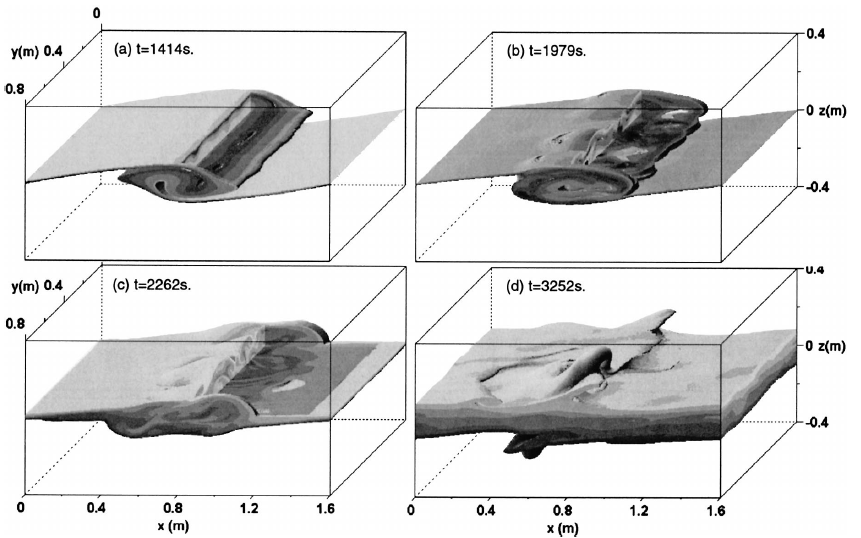
\includegraphics[width=0.9\textwidth]{kh3.png}\\
  \caption{Time evolution for a Kelvin-Helmholtz mode (Smyth and Winters \cite{Smyth})}\label{kh3}
\end{figure}
\begin{figure}[htpb]
  \centering
  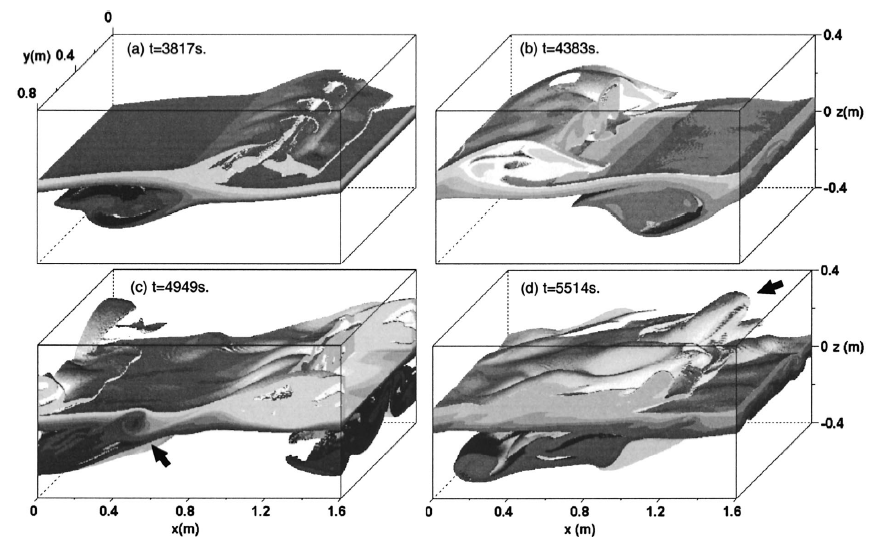
\includegraphics[width=0.9\textwidth]{ho5.png}\\
  \caption{Time evolution for a Holmboe mode (Smyth and Winters \cite{Smyth})}\label{ho5}
\end{figure}
